\documentclass[12pt, a4paper]{report}

\usepackage{graphicx}
\usepackage{float}
\usepackage{enumerate}

\usepackage{listings}

\usepackage[a4paper,left=3cm,right=2cm,top=2.5cm,bottom=2.5cm]{geometry}

\usepackage{xcolor}

\definecolor{codegreen}{rgb}{0,0.6,0}
\definecolor{codegray}{rgb}{0.5,0.5,0.5}
\definecolor{codepurple}{rgb}{0.58,0,0.82}
\definecolor{backcolour}{rgb}{0.95,0.95,0.92}

\lstdefinestyle{mystyle}{
	backgroundcolor=\color{backcolour},   
	commentstyle=\color{codegreen},
	keywordstyle=\color{magenta},
	numberstyle=\tiny\color{codegray},
	stringstyle=\color{codepurple},
	basicstyle=\ttfamily\footnotesize,
	breakatwhitespace=false,         
	breaklines=true,                 
	captionpos=b,                    
	keepspaces=true,                 
	numbers=none,                    
	numbersep=5pt,                  
	showspaces=false,                
	showstringspaces=false,
	showtabs=false,                  
	tabsize=2
}
\lstset{style=mystyle}

\usepackage[hidelinks]{hyperref}

\date{} 

\begin{document} \pagenumbering{arabic}

\begin{center}
	\bfseries 
	Experiment 1 \hfill Date: 16/07/2026
\end{center}


\begin{center}
{\bfseries \Huge Linear Regression}	
\end{center}


\section*{Aim}
Implement linear regression with one variable on the California Housing dataset to predict housing prices based on a single feature (e.g., the average number of rooms per dwelling).  \\
Tasks:
\begin{enumerate}[\quad -]
\itemsep 0em 

\item Load and preprocess the datase.
\item Implement linear regression using both gradient descent and the normal equation.
\item Evaluate the model performance using metrics such as Mean Squared Error (MSE) and R-squared.
\item Visualize the fitted line along with the data points.
\end{enumerate}

\section*{Algorithm} 

\begin{enumerate}
	\itemsep 0em
	\item \textbf{Load and Extract Data:} Load the California Housing dataset, select a single feature (e.g., \texttt{AveRooms}), and extract the target (\texttt{MedHouseVal}).
	\item \textbf{Preprocess Data:} Add a column of ones to the feature matrix to account for the intercept term and split the data into training and testing sets.
	\item \textbf{Implement Gradient Descent:} Initialize parameters, then iteratively compute predictions, calculate Mean Squared Error, find gradients, and update parameters using a chosen learning rate.
	\item \textbf{Implement Normal Equation:} Compute the optimal weights analytically using the closed-form formula: $\theta = (X^T X)^{-1} X^T y$.
	\item \textbf{Evaluate Models:} Compute performance metrics (MSE and $R^2$ score) for both the gradient descent and normal equation models.
	\item \textbf{Visualize Results:} Generate a scatter plot of the data points and overlay the fitted regression lines derived from both methods.
\end{enumerate}


\section*{Program}

\lstinputlisting[language=Python]{"./ml_lab/programs/01.py"} 

\section*{Output}

\begin{figure}[H]
	\centering
	\begin{minipage}{0.7\linewidth}
		\centering
		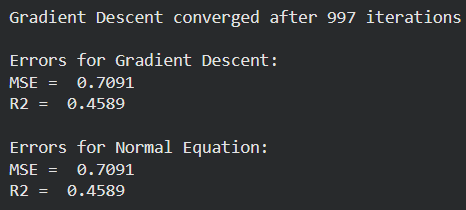
\includegraphics[width=\linewidth]{ml_lab/out/01-01}

	\end{minipage}
	\hfill
	\begin{minipage}{\linewidth}
		\centering
		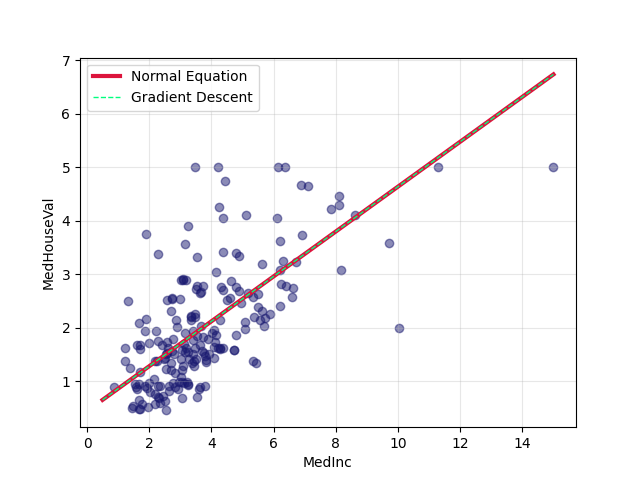
\includegraphics[width=\linewidth]{ml_lab/out/01-02}
	\end{minipage}
\end{figure}


\section*{Result} 
The linear regression model was implemented successfully using both Gradient Descent and the Normal
Equation, and the fitted regression line was also obtained 



\newpage 
\begin{center}
	\bfseries 
	Experiment 2 \hfill Date: 16/07/2026
\end{center}


\begin{center}
	{\bfseries \Huge Polynomial Regression}	
\end{center}

\section*{Aim} 

Implement polynomial regression on the Auto MPG dataset to predict miles per gallon (MPG) based on engine
displacement. Compare polynomial regression results with linear regression. \\
Tasks:
\begin{enumerate}[\quad -]
	\itemsep 0em 
	
	\item Load and preprocess the dataset.
	\item Implement polynomial regression of varying degrees.
	\item Compare the polynomial regression models with linear regression using metrics such as MSE and R-squared.
	\item Visualize the polynomial fit.
	
\end{enumerate}

\section*{Algorithm} 
\begin{enumerate}
	\itemsep 0em
	\item \textbf{Load and Preprocess Data:} Load the Auto MPG dataset, extract engine displacement as the feature and MPG as the target, handle any missing values, and split the data into training and testing sets.
	\item \textbf{Implement Linear Regression:} Fit a baseline simple linear regression model using the displacement feature.
	\item \textbf{Implement Polynomial Regression:} Generate polynomial feature expansions for varying degrees and fit regression models on these transformed features.
	\item \textbf{Evaluate and Compare Models:} Compute performance metrics (MSE and $R^2$ score) to compare the linear model with the different polynomial regression models.
	\item \textbf{Visualize the Fits:} Generate a scatter plot of the data points and overlay the curves fitted by both the linear and polynomial regression models.
\end{enumerate}

\section*{Program} 

\lstinputlisting[language=Python]{"ml_lab/programs/02.py"}

\newpage 
\section*{Output} 

\begin{figure}[H]
	\centering
	\begin{minipage}{0.7\linewidth}
		\centering
		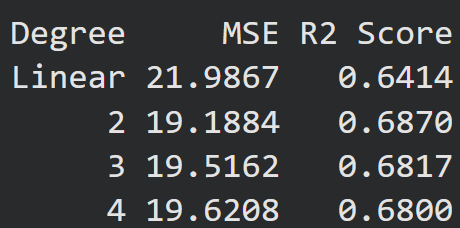
\includegraphics[width=0.5\linewidth]{ml_lab/out/02-01}
		
	\end{minipage}
	\hfill
	\begin{minipage}{\linewidth}
		\centering
		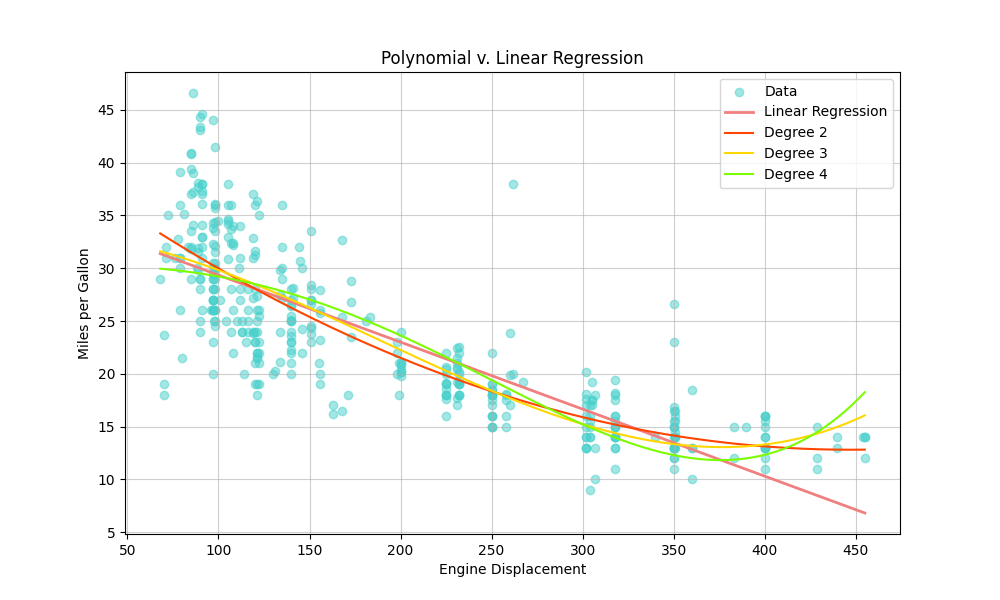
\includegraphics[width=0.7\linewidth]{ml_lab/out/02-02}
	\end{minipage}
\end{figure}


\section*{Result} 
Successfully implemented polynomial regression and compared it with linear regression on the auto MPG dataset. 


\newpage 
\begin{center}
	\bfseries 
	Experiment 3 \hfill Date: 04/08/2026 
\end{center}


\begin{center}
	{\bfseries \Huge Ridge and Lasso Regression}	
\end{center}

\section*{Aim} 
Implement Ridge and Lasso regression on the Diabetes dataset. Compare the performance of these regularized
models with standard linear regression. \\
Tasks:
\begin{enumerate}[\quad -]
	\itemsep 0em 
	
	\item Load and preprocess the dataset.
	\item Implement Ridge and Lasso regression.
	\item Tune hyperparameters using cross-validation.
	\item Compare performance metrics (MSE, R-squared) with standard linear regression.
\end{enumerate}

\section*{Algorithm} 
\begin{enumerate}
	\itemsep 0em
	\item \textbf{Load and Preprocess Data:} Load the Diabetes dataset, split it into training and testing sets, and standardize the features since regularized models are sensitive to feature scales.
	\item \textbf{Implement Standard Linear Regression:} Fit a baseline ordinary least squares linear regression model on the scaled data.
	\item \textbf{Implement Ridge and Lasso Regression:} Define Ridge (L2 penalty) and Lasso (L1 penalty) regression models.
	\item \textbf{Tune Hyperparameters:} Use cross-validation techniques to find the optimal regularization strength ($\alpha$) for both Ridge and Lasso.
	\item \textbf{Evaluate and Compare Models:} Compare performance metrics (MSE and $R^2$) of the tuned regularized models against standard linear regression.
\end{enumerate}

\section*{Program} 

\lstinputlisting[language=Python]{"ml_lab/programs/03.py"}

\newpage 
\section*{Output} 

\begin{figure}[H]
	\centering
	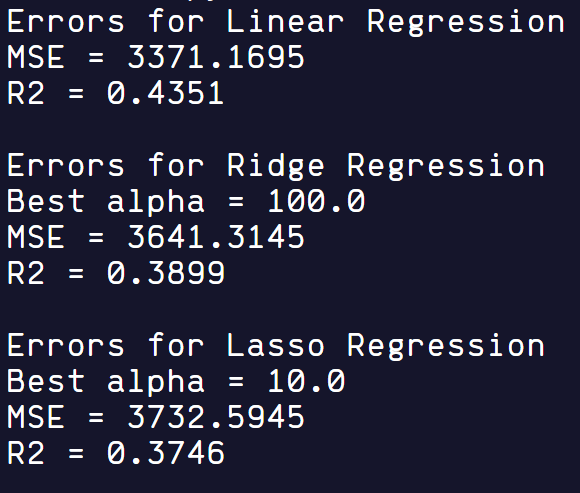
\includegraphics[width=0.5\linewidth]{ml_lab/out/03}
\end{figure}


\section*{Result} 
Successfully implemented ridge and lasso regressions on the diabetes dataset. 


\newpage 
\begin{center}
	\bfseries 
	Experiment 4 \hfill Date: 04/08/2026
\end{center}


\begin{center}
	{\bfseries \Huge Logistic Regression}	
\end{center}

\section*{Aim} 
Implement a logistic regression model to predict the likelihood of a disease using the Pima Indians Diabetes
dataset. Compare the performance with and without feature scaling. \\
Tasks:
\begin{enumerate}[\quad -]
	\itemsep 0em 
	
	\item Load and preprocess the Pima Indians Diabetes dataset.
	\item Implement logistic regression for binary classification.
	\item Evaluate model performance with and without feature scaling.
	\item Analyze metrics such as accuracy, precision, recall, and F1-score.
\end{enumerate}


\section*{Algorithm} 
\begin{enumerate}
	\itemsep 0em
	\item \textbf{Load and Preprocess Data:} Load the Diabetes dataset, split it into training and testing sets, and standardize the features since regularized models are sensitive to feature scales.
	\item \textbf{Implement Standard Linear Regression:} Fit a baseline ordinary least squares linear regression model on the scaled data.
	\item \textbf{Implement Ridge and Lasso Regression:} Define Ridge (L2 penalty) and Lasso (L1 penalty) regression models.
	\item \textbf{Tune Hyperparameters:} Use cross-validation techniques to find the optimal regularization strength ($\alpha$) for both Ridge and Lasso.
	\item \textbf{Evaluate and Compare Models:} Compare performance metrics (accuracy, precision, recall, and f1 score) of the tuned regularized models against standard linear regression.
\end{enumerate}

\section*{Program} 
\lstinputlisting[language=Python]{"ml_lab/programs/04.py"}

\newpage 
\section*{Output} 
\begin{figure}[H]
	\centering
	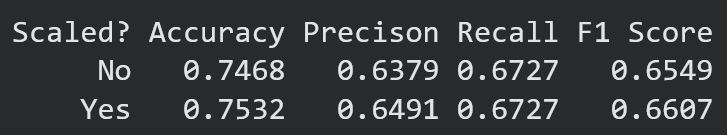
\includegraphics[width=0.5\linewidth]{ml_lab/out/04}
\end{figure}


\section*{Result} 
Successfully implemented logistic regression on the Pima Indian diabetes dataset and compared the results with and without feature scaling. 


\newpage 
\begin{center}
	\bfseries 
	Experiment 5 \hfill Date: 13/08/2026
\end{center}


\begin{center}
	{\bfseries \Huge Naive Bayes Classifier}	
\end{center}

\section*{Aim} 
Implement a Naïve Bayes classifier to categorize text documents into topics using the 20 Newsgroups dataset.
Compare the performance of Multinomial Naïve Bayes with Bernoulli Naïve Bayes. \\
Tasks:
\begin{enumerate}[\quad -]
	\itemsep 0em 
	
	\item Load and preprocess the 20 Newsgroups dataset.
	\item Implement Multinomial Naïve Bayes and Bernoulli Naïve Bayes classifiers.
	\item Evaluate and compare the performance of both models using metrics such as accuracy and F1-score.
	\item Discuss the strengths and weaknesses of each Naïve Bayes variant for text classification.
\end{enumerate}

\section*{Algorithm} 
\begin{enumerate}
	\item Load a subset of the 20 Newsgroups dataset and split into train and test sets.
	\item Preprocess text documents through lowercasing, tokenization, and stop-word removal.
	\item Vectorize text using term-frequency counts for the Multinomial variant.
	\item Binarize text features (presence or absence) for the Bernoulli variant.
	\item Train the Multinomial Naïve Bayes classifier on word-count distributions.
	\item Train the Bernoulli Naïve Bayes classifier on binary feature indicators.
	\item Evaluate both models using accuracy, precision, recall, and macro F1-scores.
	\item Compare results to demonstrate how frequency modeling benefits text classification.
\end{enumerate}

\section*{Program} 
\lstinputlisting[language=Python]{"ml_lab/programs/05.py"}

\newpage 
\section*{Output} 

\begin{figure}[H]
	\centering
	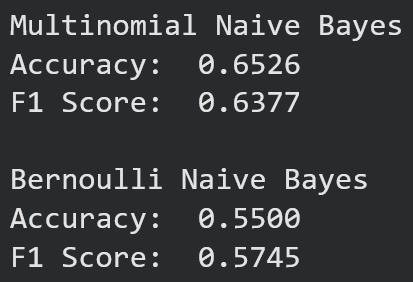
\includegraphics[width=0.5\linewidth]{ml_lab/out/05}
\end{figure}


\section*{Result} 
Successfully implemented a Naive Bayes classifier on the 20 News Groups dataset and compared the results for binary and multinomial classifiers. 


\newpage 
\begin{center}
	\bfseries 
	Experiment 6 \hfill Date: 13/08/2026
\end{center}


\begin{center}
	{\bfseries \Huge Logistic Regression With Regularization}	
\end{center}

\section*{Aim} 
Estimate the parameters of a logistic regression model using MLE and MAP on the Breast Cancer Wisconsin
dataset. Compare the results and discuss the effects of regularization. \\
Tasks:
\begin{enumerate}[\quad -]
	\itemsep 0em 
	
	\item Load and preprocess the dataset.
	\item Implement logistic regression with MLE.
	\item Apply MAP estimation with different regularization priors (L1 and L2 regularization).
	\item Compare the performance and parameter estimates with MLE and MAP.
\end{enumerate}

\section*{Algorithm} 
\begin{enumerate}
	\item Load the Breast Cancer Wisconsin dataset and split it into training and testing subsets.
	\item Standardize features to ensure fair penalty scaling during regularization.
	\item Formulate Maximum Likelihood Estimation (MLE) using unpenalized binary cross-entropy loss.
	\item Optimize MLE parameters via gradient ascent or iterative numerical solvers.
	\item Formulate Maximum A Posteriori (MAP) estimation by adding parameter priors to the objective.
	\item Implement L2 regularization (Gaussian prior) to penalize large parameter magnitudes.
	\item Implement L1 regularization (Laplacian prior) to induce parameter sparsity and feature selection.
	\item Compare test performance metrics and analyze how regularization prevents overfitting.
\end{enumerate}

\section*{Program} 
\lstinputlisting[language=Python]{"ml_lab/programs/06.py"}

\newpage 
\section*{Output} 
\begin{figure}[H]
	\centering
	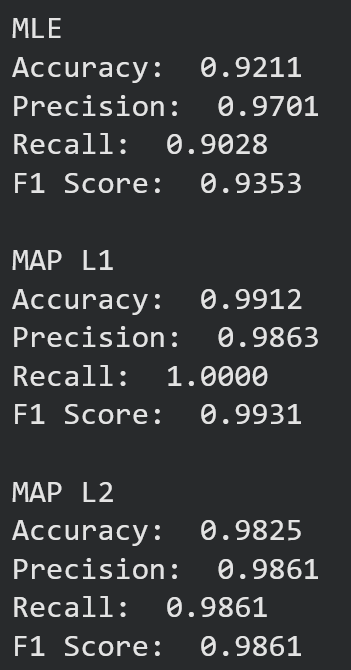
\includegraphics[width=0.5\linewidth]{ml_lab/out/06}

\end{figure}

\section*{Result} 
Successfully estimated data with MLE, L1, and L2 priors with logistic regression. 

\newpage 
\begin{center}
	\bfseries 
	Experiment 7 \hfill Date: 13/08/2026
\end{center}


\begin{center}
	{\bfseries \Huge MLE and MAP}	
\end{center}

\section*{Aim} 
Use MLE and MAP to estimate the parameters of a multinomial distribution on the 20Newsgroups dataset. Explore
the impact of different priors on the estimation. \\
Tasks:
\begin{enumerate}[\quad -]
	\itemsep 0em 
	
	\item Load and preprocess the dataset.
	\item Implement MLE for multinomial distribution parameter estimation.
	\item Apply MAP estimation with various priors (e.g., Dirichlet priors).
	\item Compare results and evaluate the effect of different priors.
\end{enumerate}

\section*{Algorithm} 
\begin{enumerate}
	\item Load a subset of the 20 Newsgroups dataset and extract text documents.
	\item Tokenize documents and construct a shared vocabulary index.
	\item Compute term frequency counts across the text corpus.
	\item Implement Maximum Likelihood Estimation (MLE) using raw relative word frequencies.
	\item Handle zero-probability issues caused by unseen words in MLE parameter estimation.
	\item Formulate Maximum A Posteriori (MAP) estimation using a conjugate Dirichlet prior.
	\item Apply Laplace smoothing (uniform Dirichlet prior) to regularize parameter estimates.
	\item Experiment with informative (non-uniform) Dirichlet priors to bias parameter weights.
	\item Compare estimated parameter distributions and evaluate the impact of different prior configurations.
\end{enumerate}

\section*{Program} 
\lstinputlisting[language=Python]{"ml_lab/programs/07.py"}

\newpage 
\section*{Output}

\begin{minipage}{\linewidth}
	\centering
	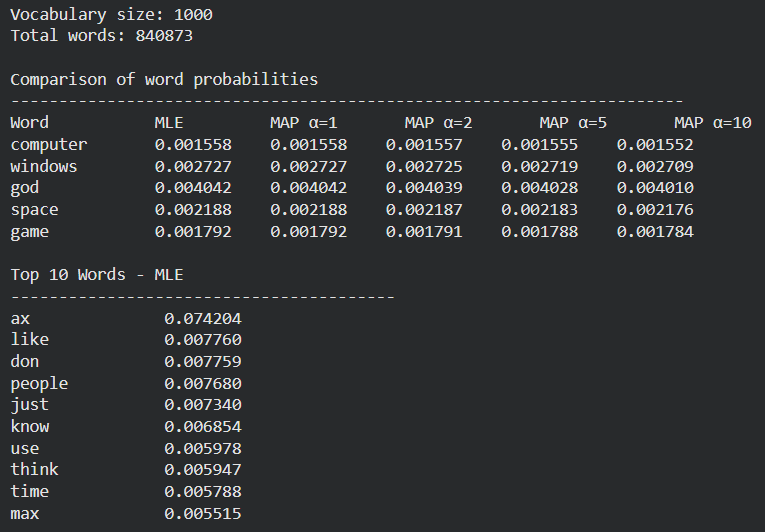
\includegraphics[width=0.7\linewidth]{ml_lab/out/07-01}
\end{minipage}
 
\begin{figure}[H]
	\centering
	\begin{minipage}{0.48\linewidth}
		\centering
		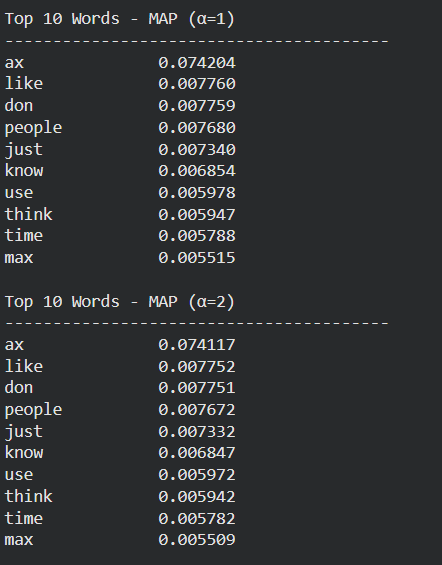
\includegraphics[width=\linewidth]{ml_lab/out/07-02}
	\end{minipage}
	\hfill 
	\begin{minipage}{0.48\linewidth}
		\centering
		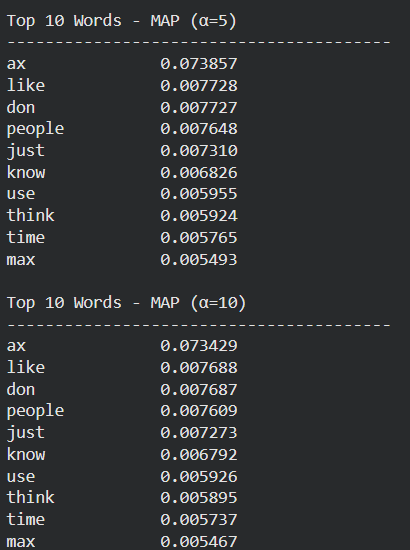
\includegraphics[width=\linewidth]{ml_lab/out/07-03}
	\end{minipage}
\end{figure}


\section*{Result} 
Successfully implemented MLE and MAP on the 20 News Groups dataset and compared effects of different priors. 



\newpage 
\begin{center}
	\bfseries 
	Experiment 8 \hfill Date: 01/09/2026
\end{center}


\begin{center}
	{\bfseries \Huge K Nearest Neighbors}	
\end{center}

\section*{Aim} 
Implement the K-Nearest Neighbors (KNN) algorithm for image classification using the Fashion MNIST dataset.
Experiment with different values of K and analyze their impact
on model performance. \\
Tasks:
\begin{enumerate}[\quad -]
	\itemsep 0em 
	
	\item Load and preprocess the Fashion MNIST dataset.
	\item Implement KNN for multi-class classification.
	\item Experiment with different values of K and evaluate performance.
	\item Discuss the impact of different K values on model accuracy and computational efficiency.
\end{enumerate}

\section*{Algorithm} 
\begin{enumerate}
	\item Load the Fashion MNIST dataset containing 28x28 grayscale clothing images.
	\item Normalize pixel intensity values to a standard range (e.g., $[0, 1]$).
	\item Flatten 2D image matrices into 1D feature vectors for distance computation.
	\item Sample a manageable subset of the dataset to mitigate KNN's high computational complexity during inference.
	\item Split the preprocessed data into training and testing sets.
	\item Implement the K-Nearest Neighbors classifier using distance metrics like Euclidean distance.
	\item Train models across a range of different $K$ values (e.g., $1, 3, 5, 11$).
	\item Evaluate classification performance using accuracy, precision, and recall metrics for each $K$.
	\item Analyze how small $K$ leads to overfitting (high variance) and large $K$ leads to underfitting (high bias).
	\item Discuss the computational trade-offs and slow inference times associated with lazy learning algorithms.
\end{enumerate}

\section*{Program} 
\lstinputlisting[language=Python]{"ml_lab/programs/08.py"}

\newpage 
\section*{Output} 

\begin{figure}[H]
	\centering
	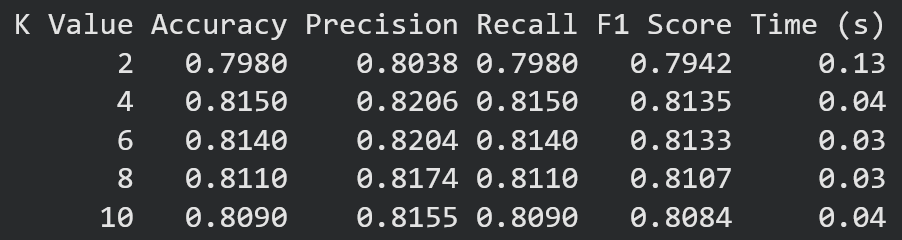
\includegraphics[width=0.5\linewidth]{ml_lab/out/08}
\end{figure}


\section*{Result} 
Successfully implemented KNN on the Fashion MNIST dataset and compared different k-values. 

\newpage 
\begin{center}
	\bfseries 
	Experiment 9 \hfill Date: 01/09/2026
\end{center}


\begin{center}
	{\bfseries \Huge Iterative Dichotomiser 3 Algorithm}	
\end{center}

\section*{Aim} 
Implement a Decision Tree classifier using the ID3 algorithm to segment customers based on their purchasing
behavior using the Iris dataset. Analyze the tree structure
and discuss the feature importance. \\
Tasks:
\begin{enumerate}[\quad -]
	\itemsep 0em 
	
	\item Load and preprocess the Iris dataset.
	\item Implement Decision Tree using the ID3 algorithm.
	\item Visualize the decision tree and analyze feature importance.
	\item Discuss how the tree structure helps in understanding customer behavior.
\end{enumerate}

\section*{Algorithm} 
\begin{enumerate}
	\item Load the preprocessed dataset and ensure all feature attributes are discretized into categorical values.
	\item Compute the total entropy of the dataset based on the class distribution of the target variable.
	\item For each available feature, calculate the conditional entropy after splitting the dataset on that feature's attributes.
	\item Compute the Information Gain for each feature by subtracting its conditional entropy from the total dataset entropy.
	\item Select the feature that yields the maximum Information Gain to be the current decision node.
	\item Partition the dataset into subsets corresponding to the discrete branches of the selected feature.
	\item Recursively repeat the entropy and information gain calculations for each subset to construct child nodes.
	\item Terminate recursion when all instances in a node belong to a single target class or when no remaining features are left.
	\item Output the fully constructed decision tree structure to analyze split paths and evaluate feature importance.
\end{enumerate}

\section*{Program} 
\lstinputlisting[language=Python]{"ml_lab/programs/09.py"}

\newpage 
\section*{Output} 

\begin{figure}[H]
	\centering
	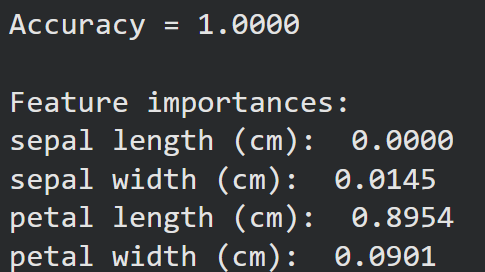
\includegraphics[width=0.4\linewidth]{ml_lab/out/09-01}
\end{figure}
\begin{figure}[H]
	\centering
	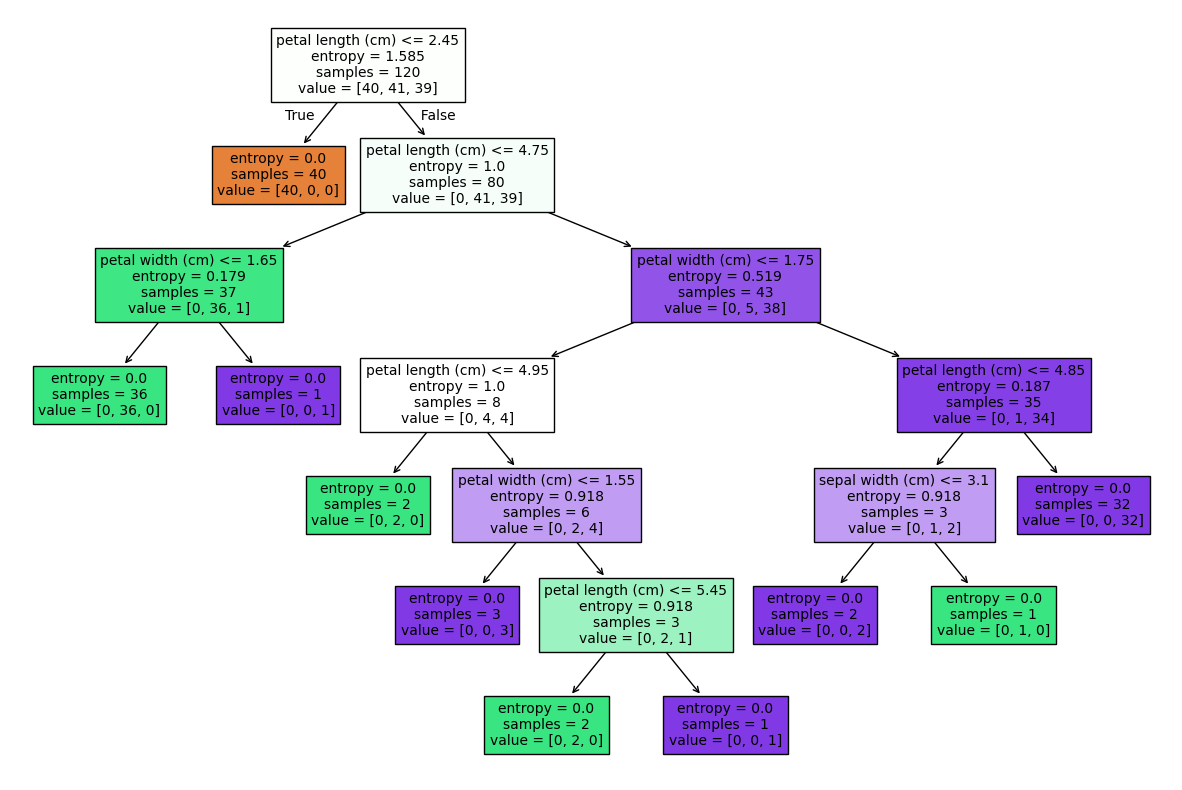
\includegraphics[width=0.9\linewidth]{ml_lab/out/09-02}
\end{figure}


\section*{Result} 
Successfully implemented the ID3 algorithm on the Iris dataset. 

\newpage 
\begin{center}
	\bfseries 
	Experiment 10 \hfill Date: 08/09/2026
\end{center}


\begin{center}
	{\bfseries \Huge Support Vector Machines}	
\end{center}

\section*{Aim} 
Implement a Linear Support Vector Machine (SVM) to classify the Iris dataset. Visualize the decision boundary
and discuss how the margin is determined. \\
Tasks:
\begin{enumerate}[\quad -]
	\itemsep 0em 
	
	\item Load and preprocess the Iris dataset.
	\item Implement a Linear SVM for binary classification (e.g., classify Setosa vs. Non-Setosa).
	\item Visualize the decision boundary and margin.
	Discuss the concept of the margin and how it influences classification.
\end{enumerate}


\section*{Algorithm} 
\begin{enumerate}
	\item Load the Iris dataset, select two features for 2D visualization, and filter for binary classification.
	\item Standardize the feature values and split the data into training and testing sets.
	\item Formulate the linear SVM optimization problem to maximize the margin subject to classification constraints.
	\item Train the linear SVM model to find the optimal hyperplane and identify the support vectors.
	\item Visualize the decision boundary, the margin boundaries, and the support vectors alongside the data points.
	\item Analyze how the margin width and the regularization parameter influence the model's performance.
\end{enumerate}

\section*{Program} 
\lstinputlisting[language=Python]{"ml_lab/programs/10.py"}

\newpage 
\section*{Output} 

\begin{figure}[H]
	\centering
	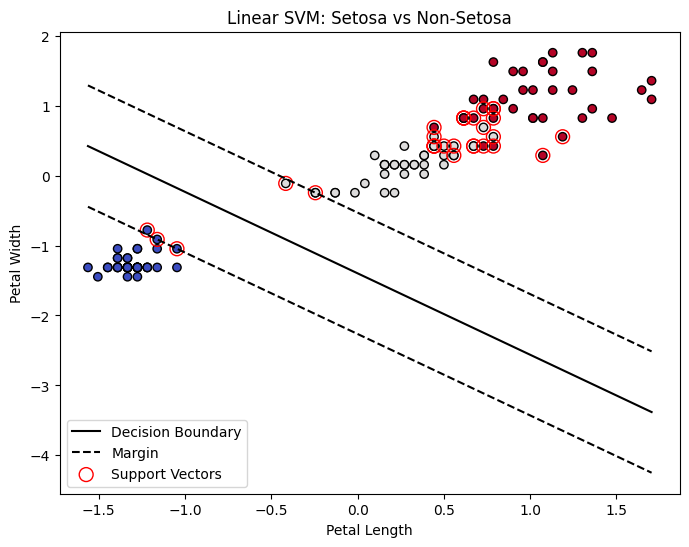
\includegraphics[width=0.7\linewidth]{ml_lab/out/10-02}
\end{figure}

\section*{Result} 
Successfully classified data into setosa and non-setosa classes using a linear SVM on the Iris dataset. 


\newpage 
\begin{center}
	\bfseries 
	Experiment 11 \hfill Date: 15/09/2026
\end{center}


\begin{center}
	{\bfseries \Huge SVM Kernels}	
\end{center}

\section*{Aim} 
Implement and compare the performance of SVM classifiers with linear, polynomial, and RBF kernels on the
Fashion MNIST dataset. Analyze the advantages and disadvantages of
each kernel type. \\
Tasks:
\begin{enumerate}[\quad -]
	\itemsep 0em 
	
	\item Load and preprocess the Fashion MNIST dataset.
	\item Implement SVM with linear, polynomial, and RBF kernels.
	\item Compare the classification performance for each kernel.
	\item Discuss the strengths and weaknesses of each kernel type.
	
\end{enumerate}


\section*{Algorithm} 
\begin{enumerate}
	\item Load the Fashion MNIST dataset and normalize pixel intensity values to the range $[0, 1]$.
	\item Flatten the 2D image matrices into 1D feature vectors and split into training and testing sets.
	\item Implement a Support Vector Machine using a linear kernel to construct flat decision boundaries.
	\item Implement an SVM with a polynomial kernel to capture non-linear feature interactions.
	\item Implement an SVM with a Radial Basis Function (RBF) kernel to map inputs into infinite-dimensional space.
	\item Train all three kernel variants and evaluate their classification performance using accuracy, precision, recall, and F1-score metrics.
	\item Analyze strengths and weaknesses: note that linear kernels are fast but underfit complex shapes, polynomial kernels risk high computational costs and overfitting, and RBF kernels handle intricate boundaries effectively at the expense of heavy memory and training time.
\end{enumerate}


\section*{Program} 
\lstinputlisting[language=Python]{"ml_lab/programs/11.py"}

\newpage 
\section*{Output} 

\begin{figure}[H]
	\centering
	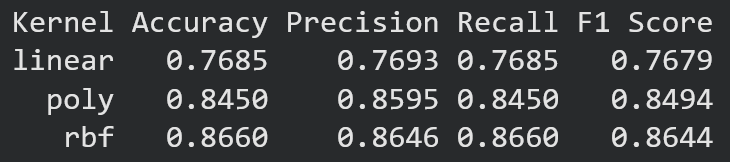
\includegraphics[width=0.7\linewidth]{ml_lab/out/11}
\end{figure}


\section*{Result} 
Successfully implemented support vector machines with linear, polynomial (degree=3), and RBF kernels on the Fashion MNIST dataset. 


\newpage 
\begin{center}
	\bfseries 
	Experiment 12 \hfill Date: 15/09/2026
\end{center}


\begin{center}
	{\bfseries \Huge Multilayer Feed-Forward Networks}	
\end{center}

\section*{Aim} 
Implement and train a Multilayer Feed-Forward Network (MLP) on the Wine Quality dataset. Experiment with
different numbers of hidden layers and neurons, and discuss how these choices affect the network’s performance.\\
Tasks:
\begin{enumerate}[\quad -]
	\itemsep 0em 
	
	\item Load and preprocess the Wine Quality dataset.
	\item Design and implement an MLP with varying architectures (different hidden layers and neurons).
	\item Train and evaluate the network.
	\item Discuss the impact of architecture choices on performance.
	
\end{enumerate}


\section*{Algorithm} 
\begin{enumerate}
	\item Load the Wine Quality dataset, handle missing values, and split into training and testing sets.
	\item Standardize input features to ensure stable gradient descent and faster convergence during backpropagation.
	\item Design a baseline Multilayer Feed-Forward Network (MLP) featuring input, hidden, and output layers.
	\item Configure appropriate loss functions, activation functions (e.g., ReLU), and optimizers (e.g., Adam).
	\item Train multiple network variants with varying depths (different numbers of hidden layers) and widths (different neuron counts).
	\item Evaluate performance using relevant metrics (e.g., accuracy, F1-score, or mean squared error).
	\item Discuss how architectural choices affect model capacity, risk of overfitting, and generalization capabilities.
\end{enumerate}

\section*{Program} 
\lstinputlisting[language=Python]{"ml_lab/programs/12.py"}

\newpage 
\section*{Output} 

\begin{figure}[H]
	\centering
	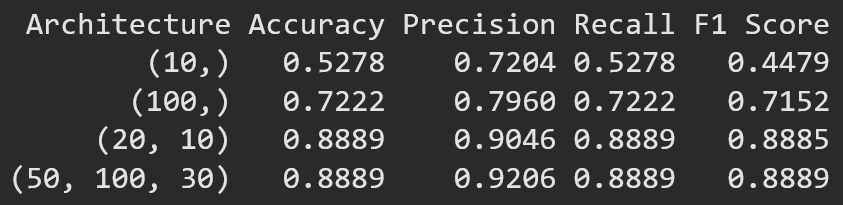
\includegraphics[width=0.7\linewidth]{ml_lab/out/12}
\end{figure}



\section*{Result} 
Successfully implemented multilayer feed-forward networks on the Wine Quality dataset and compared the performance of different architectures. 


\newpage 
\begin{center}
	\bfseries 
	Experiment 13 \hfill Date: 15/09/2026
\end{center}


\begin{center}
	{\bfseries \Huge Neural Networks}	
\end{center}

\section*{Aim} 
Implement and compare the performance of a neural network using different activation functions (Sigmoid, ReLU,
Tanh) on the MNIST dataset. Analyze how each activation function affects the training process and classification
accuracy.\\
Tasks:
\begin{enumerate}[\quad -]
	\itemsep 0em 
	
	\item Load and preprocess the MNIST dataset.
	\item Implement neural networks using Sigmoid, ReLU, and Tanh activation functions.
	\item Train and evaluate each network.
	\item Compare training times, convergence, and classification accuracy.
	
\end{enumerate}


\section*{Algorithm} 
\begin{enumerate}
	\item Load the MNIST dataset and scale pixel intensity values to the range $[0, 1]$.
	\item Flatten the 2D image matrices into 1D feature vectors and split into training and testing sets.
	\item Build a baseline neural network architecture with configurable hidden layers and a softmax output layer.
	\item Implement the Sigmoid activation function to map hidden layer outputs to the range $(0, 1)$.
	\item Implement the Tanh activation function to map hidden layer outputs to a zero-centered range $(-1, 1)$.
	\item Implement the ReLU (Rectified Linear Unit) activation function to output positive values directly while thresholding negatives.
	\item Train each network variant independently using identical hyperparameter configurations and optimizers.
	\item Compare training times, convergence rates, and test classification accuracies.
	\item Analyze how Sigmoid and Tanh suffer from vanishing gradients while ReLU enables faster and deeper convergence.
\end{enumerate}


\section*{Program} 
\lstinputlisting[language=Python]{"ml_lab/programs/13.py"}

\newpage 
\section*{Output} 

\begin{figure}[H]
	\centering
	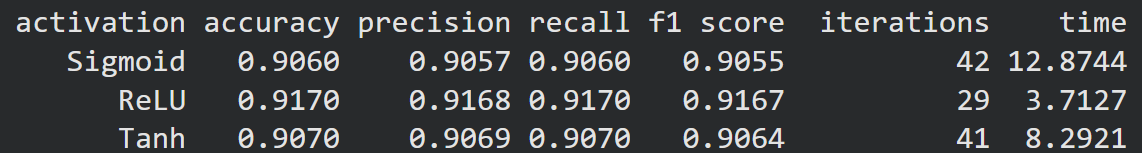
\includegraphics[width=\linewidth]{ml_lab/out/13}
\end{figure}


\section*{Result} 
Successfully implemented and compared the performances of neural networks with Sigmoid, ReLU, and Tanh activation functions on the MNIST dataset. 


\newpage 
\begin{center}
	\bfseries 
	Experiment 14 \hfill Date: 24/09/2026
\end{center}


\begin{center}
	{\bfseries \Huge Hierarchical and Partitional Clustering}	
\end{center}

\section*{Aim} 
Implement and compare hierarchical (agglomerative) and partitional (K-means) clustering algorithms on the Mall
Customers dataset. Discuss the strengths and weaknesses of each method based on clustering results and evaluation
metrics.\\
Tasks:
\begin{enumerate}[\quad -]
	\itemsep 0em 
	
	\item Load and preprocess the Mall Customers dataset.
	\item Apply both hierarchical (agglomerative) and K-means clustering.
	\item Compare results using metrics such as inertia, silhouette score, and clustering visualization.
	\item Discuss the advantages and disadvantages of each clustering method.
\end{enumerate}

\section*{Algorithm} 
\begin{enumerate}
	\item Load the Mall Customers dataset and select relevant features for customer segmentation.
	\item Standardize feature values to ensure equal weighting during distance calculations.
	\item Implement K-means clustering, determining the optimal number of clusters ($k$) via the Elbow method.
	\item Implement Agglomerative Hierarchical clustering using linkage criteria.
	\item Evaluate both models using Silhouette scores and cluster inertia.
	\item Visualize the resulting clusters using 2D scatter plots.
	\item Compare strengths and weaknesses: note K-means' computational efficiency versus hierarchical clustering's intuitive tree-based structures and lack of a pre-defined $k$ requirement.
\end{enumerate}

\section*{Program} 
\lstinputlisting[language=Python]{"ml_lab/programs/14.py"}

\newpage 
\section*{Output} 

\begin{figure}[H]
	\centering
	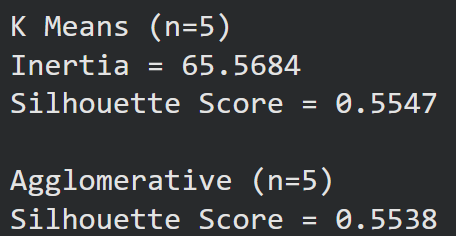
\includegraphics[width=0.5\linewidth]{ml_lab/out/14-01}
	
\end{figure}

\begin{figure}[H]
	\centering
	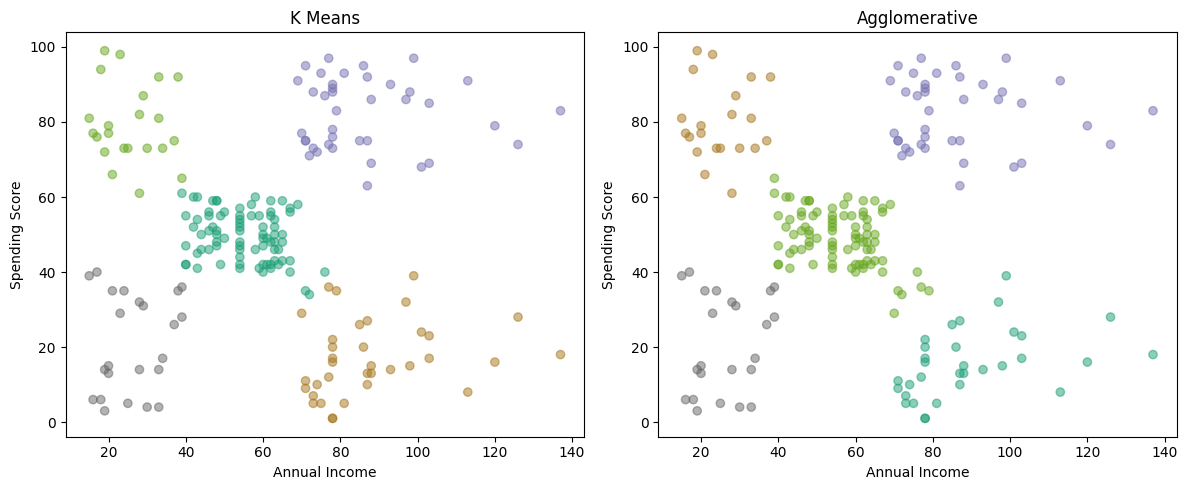
\includegraphics[width=\linewidth]{ml_lab/out/14-02}
\end{figure}



\section*{Result} 
Successfully implemented partitional (K Means) and hierarchical (agglomerative) clustering on the Mall Customers dataset. 


\newpage 
\begin{center}
	\bfseries 
	Experiment 15 \hfill Date:  24/09/2026
\end{center}


\begin{center}
	{\bfseries \Huge K-Means Clustering}	
\end{center}

\section*{Aim} 
Implement and apply K-means clustering to the Digits dataset. Experiment with different numbers of clusters and
evaluate the clustering results using metrics such as inertia and silhouette score. Analyze how the choice of K
affects clustering performance.\\
Tasks:
\begin{enumerate}[\quad -]
	\itemsep 0em 
	
	\item Load and preprocess the Digits dataset.
	\item Implement K-means clustering with various numbers of clusters.
	\item Evaluate clustering performance using inertia and silhouette score.
	\item Analyze the impact of the number of clusters on clustering quality.
\end{enumerate}


\section*{Algorithm} 
\begin{enumerate}
	\item Load the Digits dataset and normalize feature values to scale pixel intensities consistently.
	\item Implement K-means clustering across a range of different cluster counts ($K$).
	\item Compute cluster inertia (within-cluster sum of squares) for each $K$ to apply the Elbow method.
	\item Calculate Silhouette scores for each $K$ to measure cluster cohesion and separation quality.
	\item Evaluate the alignment between unsupervised clusters and true digit labels using external validation metrics if applicable.
	\item Analyze how the choice of $K$ impacts clustering performance and trade-offs between granularity and grouping error.
\end{enumerate}

\section*{Program} 
\lstinputlisting[language=Python]{"ml_lab/programs/15.py"}

\newpage 
\section*{Output} 

\begin{figure}[H]
	\centering
	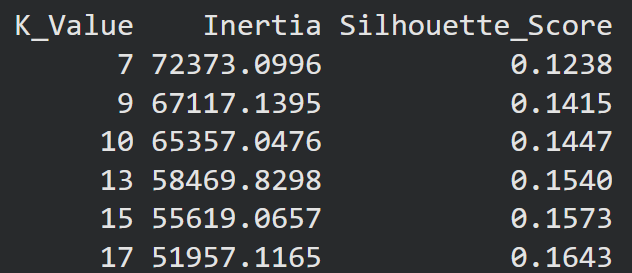
\includegraphics[width=0.5\linewidth]{ml_lab/out/15-01}
\end{figure}
\begin{figure}[H]
	\centering
	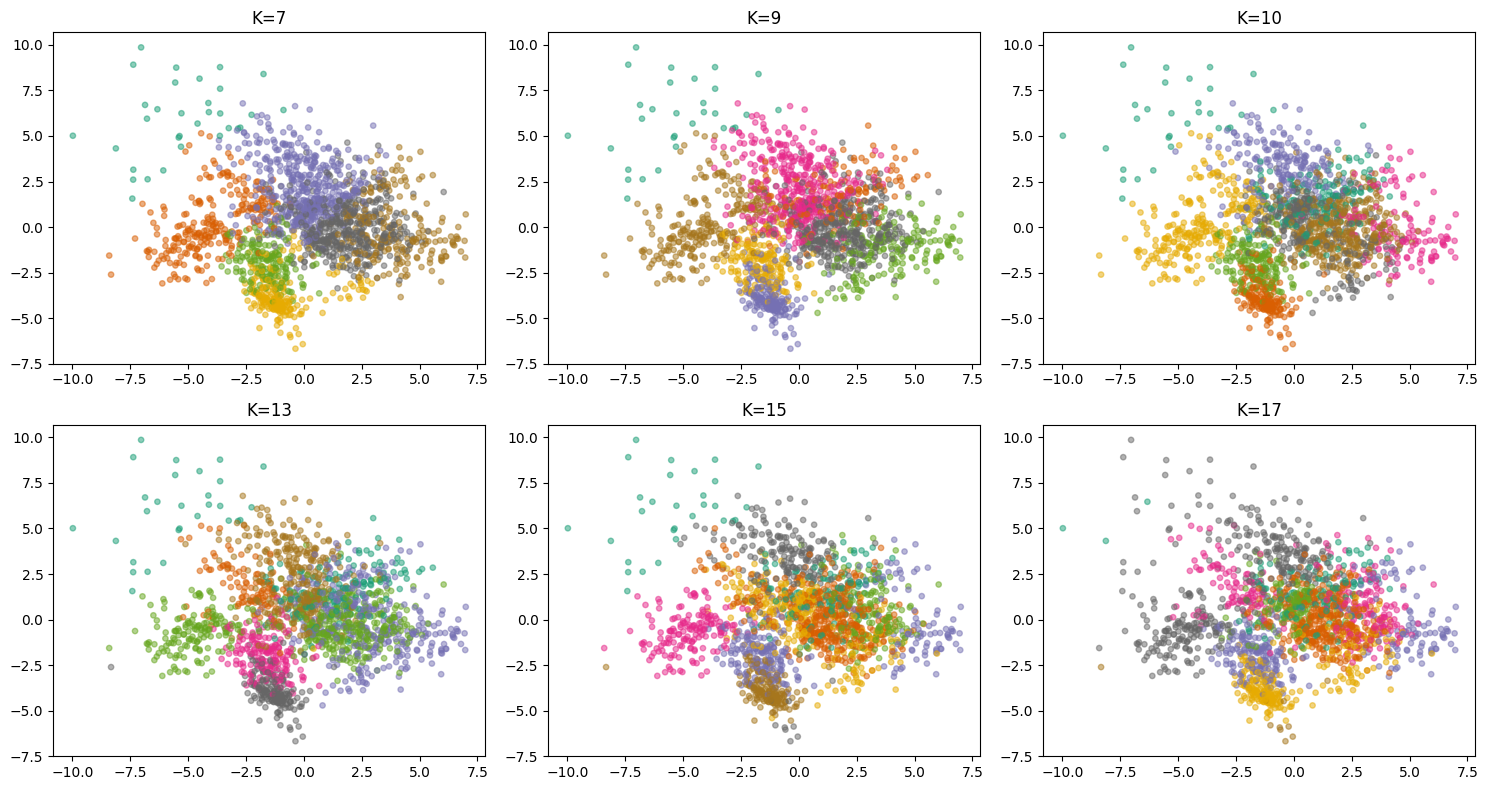
\includegraphics[width=\linewidth]{ml_lab/out/15-02}
\end{figure}


\section*{Result} 
Successfully implemented K-means clustering on the digits dataset and compared performances for different values of K. 


\newpage 
\begin{center}
	\bfseries 
	Experiment 16 \hfill Date:  24/09/2026
\end{center}


\begin{center}
	{\bfseries \Huge Bootstrapping and Cross-Validation}	
\end{center}

\section*{Aim} 
Implement bootstrapping and cross-validation on the Iris dataset. Compare the model performance metrics (e.g.,
accuracy, F1-score) obtained using these resampling methods. Discuss the advantages and disadvantages of each
method.\\
Tasks:
\begin{enumerate}[\quad -]
	\itemsep 0em 
	
	\item Load and preprocess the Iris dataset.
	\item Implement bootstrapping to generate multiple samples and evaluate the model.
	\item Implement k-fold cross-validation and evaluate the model.
	\item Compare the performance metrics and discuss the pros and cons of each resampling method.
\end{enumerate}


\section*{Algorithm} 

\begin{enumerate}
	\item Load and preprocess the Iris dataset to prepare feature matrices and target class labels.
	\item Initialize a base classification model (e.g., K-Nearest Neighbors or Logistic Regression).
	\item Implement bootstrapping by repeatedly sampling the dataset with replacement to create training sets.
	\item Evaluate the model on out-of-bag (OOB) samples or held-out validation subsets for each bootstrap iteration.
	\item Implement $k$-fold cross-validation by partitioning the dataset into $k$ mutually exclusive folds.
	\item Train and test the model iteratively across all folds, ensuring each subset serves as the validation set once.
	\item Compute and record performance metrics (e.g., accuracy, F1-score) for both resampling methods.
	\item Compare results and discuss trade-offs: bootstrapping utilizes sampling with replacement to handle small datasets but can introduce optimism bias, whereas $k$-fold cross-validation provides more reliable, unbiased error estimation.
\end{enumerate}

\section*{Program} 
\lstinputlisting[language=Python]{"ml_lab/programs/16.py"}

\newpage 
\section*{Output} 

\begin{figure}[H]
	\centering
	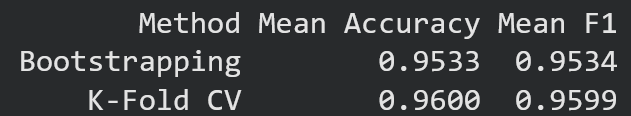
\includegraphics[width=0.7\linewidth]{ml_lab/out/16}
\end{figure}


\section*{Result} 
Successfully implemented bootstrapping and cross-validation (5-fold) on the Iris dataset. 


\newpage 
\begin{center}
	\bfseries 
	Experiment 17 \hfill Date:  24/09/2026
\end{center}


\begin{center}
	{\bfseries \Huge Bagging and Boosting}	
\end{center}

\section*{Aim} 
Implement bagging and boosting ensemble methods on the Titanic dataset. Compare the performance of both
methods in terms of accuracy, precision, recall, and F1-score. Discuss how each method improves model
performance and their respective strengths and weaknesses.\\
Tasks:
\begin{enumerate}[\quad -]
	\itemsep 0em 
	
	\item Load and preprocess the Titanic dataset.
	\item Implement bagging using a base classifier (e.g., decision tree) and evaluate performance.
	\item Implement boosting using a boosting algorithm (e.g., AdaBoost) and evaluate performance.
	\item Compare performance metrics and discuss the strengths and weaknesses of each method.
\end{enumerate}

\section*{Algorithm} 
\begin{enumerate}
	\item Load the Titanic dataset, handle missing values, encode categorical features, and split into training and testing subsets.
	\item Implement a bagging ensemble (e.g., Bagged Decision Trees or Random Forest) using bootstrap sampling with replacement to train parallel base learners.
	\item Implement a boosting ensemble (e.g., AdaBoost or Gradient Boosting) to train sequential base learners that focus on previously misclassified instances.
	\item Train both ensemble models on the training data.
	\item Evaluate model performance using accuracy, precision, recall, and F1-score metrics on the test set.
	\item Compare results and discuss how bagging primarily reduces variance while boosting reduces bias, noting their trade-offs regarding computational cost and noise sensitivity.
\end{enumerate}

\section*{Program} 
\lstinputlisting[language=Python]{"ml_lab/programs/17.py"}

\newpage 
\section*{Output} 

\begin{figure}[H]
	\centering
	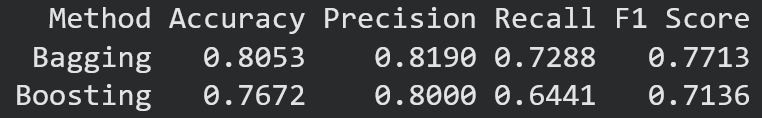
\includegraphics[width=0.7\linewidth]{ml_lab/out/17}
\end{figure}

\section*{Result} 
Successfully implemented bagging and boosting on the Titanic dataset. 


\newpage 
\begin{center}
	\bfseries 
	Experiment 18 \hfill Date:  24/09/2026
\end{center}


\begin{center}
	{\bfseries \Huge Bias-Variance Tradeoff}	
\end{center}

\section*{Aim} 
Investigate the bias-variance tradeoff using polynomial regression on the Boston Housing dataset. Plot the training
and validation errors for various polynomial degrees and discuss
the tradeoff between bias and variance.\\
Tasks:
\begin{enumerate}[\quad -]
	\itemsep 0em 
	
	\item Load and preprocess the Boston Housing dataset.
	\item Implement polynomial regression with varying degrees.Plot training and validation errors for each degree.
	\item Discuss the bias-variance tradeoff and its impact on model performance.
	
\end{enumerate}

\section*{Algorithm} 
\begin{enumerate}
	\item Load the Boston Housing dataset, handle missing values, and split into training and validation subsets.
	\item Standardize input features to prevent numerical instability with higher-order polynomial terms.
	\item Generate polynomial feature transformations across a range of increasing degrees (e.g., $d = 1$ to $d = 10$).
	\item Fit polynomial regression models on the training set for each respective degree.
	\item Compute training and validation errors (e.g., Mean Squared Error) for each model configuration.
	\item Plot training and validation errors as a function of model complexity (polynomial degree).
	\item Analyze the bias-variance tradeoff: low degrees exhibit high bias and underfitting, high degrees exhibit high variance and overfitting, and an optimal intermediate degree minimizes generalization error.
\end{enumerate}

\section*{Program} 
\lstinputlisting[language=Python]{"ml_lab/programs/18.py"}

\newpage 
\section*{Output} 

\begin{figure}[H]
	\centering
	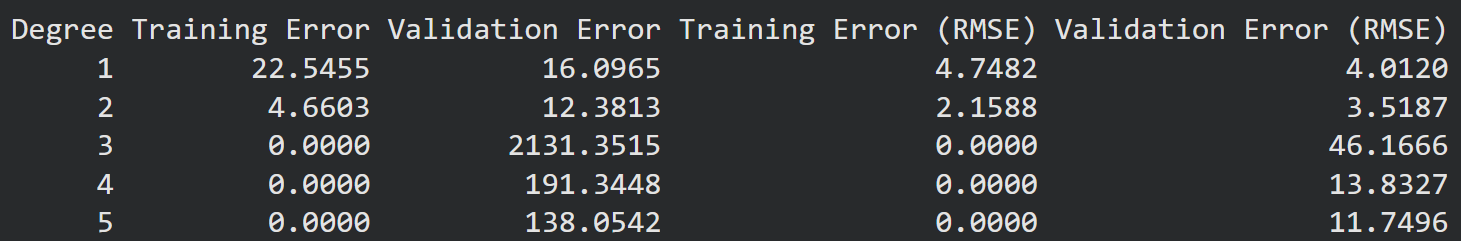
\includegraphics[width=0.9\linewidth]{ml_lab/out/18-01}
\end{figure}
\begin{figure}[H]
	\centering
	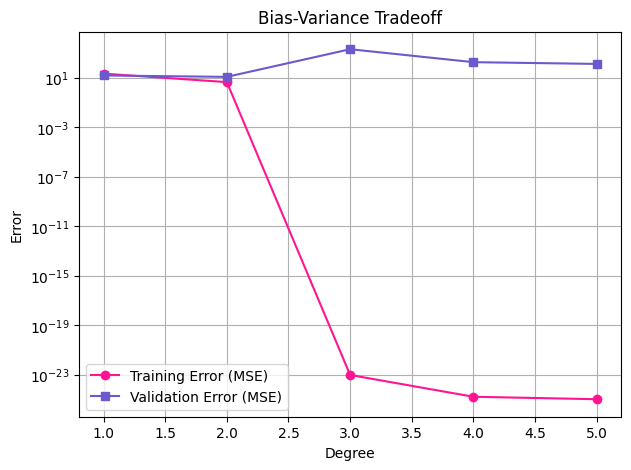
\includegraphics[width=0.5\linewidth]{ml_lab/out/18-02}
\end{figure}

\section*{Result} 
Successfully investigated the bias-variance tradeoff using polynomial regression on the Boston Housing dataset. 




\end{document}